\documentclass[11pt,]{tufte-handout}

% ams
\usepackage{amssymb,amsmath}

\usepackage{ifxetex,ifluatex}
\usepackage{fixltx2e} % provides \textsubscript
\ifnum 0\ifxetex 1\fi\ifluatex 1\fi=0 % if pdftex
  \usepackage[T1]{fontenc}
  \usepackage[utf8]{inputenc}
\else % if luatex or xelatex
  \makeatletter
  \@ifpackageloaded{fontspec}{}{\usepackage{fontspec}}
  \makeatother
  \defaultfontfeatures{Ligatures=TeX,Scale=MatchLowercase}
  \makeatletter
  \@ifpackageloaded{soul}{
     \renewcommand\allcapsspacing[1]{{\addfontfeature{LetterSpace=15}#1}}
     \renewcommand\smallcapsspacing[1]{{\addfontfeature{LetterSpace=10}#1}}
   }{}
  \makeatother
\fi

% graphix
\usepackage{graphicx}
\setkeys{Gin}{width=\linewidth,totalheight=\textheight,keepaspectratio}

% booktabs
\usepackage{booktabs}

% url
\usepackage{url}

% hyperref
\usepackage{hyperref}

% units.
\usepackage{units}


\setcounter{secnumdepth}{-1}

% citations
\usepackage{natbib}
\bibliographystyle{plainnat}

% pandoc syntax highlighting
\usepackage{color}
\usepackage{fancyvrb}
\newcommand{\VerbBar}{|}
\newcommand{\VERB}{\Verb[commandchars=\\\{\}]}
\DefineVerbatimEnvironment{Highlighting}{Verbatim}{commandchars=\\\{\}}
% Add ',fontsize=\small' for more characters per line
\newenvironment{Shaded}{}{}
\newcommand{\KeywordTok}[1]{\textcolor[rgb]{0.00,0.44,0.13}{\textbf{{#1}}}}
\newcommand{\DataTypeTok}[1]{\textcolor[rgb]{0.56,0.13,0.00}{{#1}}}
\newcommand{\DecValTok}[1]{\textcolor[rgb]{0.25,0.63,0.44}{{#1}}}
\newcommand{\BaseNTok}[1]{\textcolor[rgb]{0.25,0.63,0.44}{{#1}}}
\newcommand{\FloatTok}[1]{\textcolor[rgb]{0.25,0.63,0.44}{{#1}}}
\newcommand{\ConstantTok}[1]{\textcolor[rgb]{0.53,0.00,0.00}{{#1}}}
\newcommand{\CharTok}[1]{\textcolor[rgb]{0.25,0.44,0.63}{{#1}}}
\newcommand{\SpecialCharTok}[1]{\textcolor[rgb]{0.25,0.44,0.63}{{#1}}}
\newcommand{\StringTok}[1]{\textcolor[rgb]{0.25,0.44,0.63}{{#1}}}
\newcommand{\VerbatimStringTok}[1]{\textcolor[rgb]{0.25,0.44,0.63}{{#1}}}
\newcommand{\SpecialStringTok}[1]{\textcolor[rgb]{0.73,0.40,0.53}{{#1}}}
\newcommand{\ImportTok}[1]{{#1}}
\newcommand{\CommentTok}[1]{\textcolor[rgb]{0.38,0.63,0.69}{\textit{{#1}}}}
\newcommand{\DocumentationTok}[1]{\textcolor[rgb]{0.73,0.13,0.13}{\textit{{#1}}}}
\newcommand{\AnnotationTok}[1]{\textcolor[rgb]{0.38,0.63,0.69}{\textbf{\textit{{#1}}}}}
\newcommand{\CommentVarTok}[1]{\textcolor[rgb]{0.38,0.63,0.69}{\textbf{\textit{{#1}}}}}
\newcommand{\OtherTok}[1]{\textcolor[rgb]{0.00,0.44,0.13}{{#1}}}
\newcommand{\FunctionTok}[1]{\textcolor[rgb]{0.02,0.16,0.49}{{#1}}}
\newcommand{\VariableTok}[1]{\textcolor[rgb]{0.10,0.09,0.49}{{#1}}}
\newcommand{\ControlFlowTok}[1]{\textcolor[rgb]{0.00,0.44,0.13}{\textbf{{#1}}}}
\newcommand{\OperatorTok}[1]{\textcolor[rgb]{0.40,0.40,0.40}{{#1}}}
\newcommand{\BuiltInTok}[1]{{#1}}
\newcommand{\ExtensionTok}[1]{{#1}}
\newcommand{\PreprocessorTok}[1]{\textcolor[rgb]{0.74,0.48,0.00}{{#1}}}
\newcommand{\AttributeTok}[1]{\textcolor[rgb]{0.49,0.56,0.16}{{#1}}}
\newcommand{\RegionMarkerTok}[1]{{#1}}
\newcommand{\InformationTok}[1]{\textcolor[rgb]{0.38,0.63,0.69}{\textbf{\textit{{#1}}}}}
\newcommand{\WarningTok}[1]{\textcolor[rgb]{0.38,0.63,0.69}{\textbf{\textit{{#1}}}}}
\newcommand{\AlertTok}[1]{\textcolor[rgb]{1.00,0.00,0.00}{\textbf{{#1}}}}
\newcommand{\ErrorTok}[1]{\textcolor[rgb]{1.00,0.00,0.00}{\textbf{{#1}}}}
\newcommand{\NormalTok}[1]{{#1}}

% longtable

% multiplecol
\usepackage{multicol}

% strikeout
\usepackage[normalem]{ulem}

% morefloats
\usepackage{morefloats}


% tightlist macro required by pandoc >= 1.14
\providecommand{\tightlist}{%
  \setlength{\itemsep}{0pt}\setlength{\parskip}{0pt}}

% title / author / date
\title{West Mediterranean during the Last Deglaciation}
\author{Nick Gauthier}
\date{2016-12-12}


\begin{document}

\maketitle




\section{Introduction}\label{introduction}

We'll be comparing paleoclimate model estimates of temperature and
precipitation over three points in the west Mediterranean to global
paleoclimate proxies.

\subsection{Setup}\label{setup}

Load all the packages we'll need for this analysis.

\marginnote{You'll need to have the netCDF libraries already installed on your system for ncdf4 to work.}

\begin{Shaded}
\begin{Highlighting}[]
\KeywordTok{library}\NormalTok{(ncdf4) }\CommentTok{# import GCM data}
\KeywordTok{library}\NormalTok{(rgdal) }\CommentTok{# read GCM data}
\KeywordTok{library}\NormalTok{(raster) }\CommentTok{# process GCM data}
\KeywordTok{library}\NormalTok{(rasterVis) }\CommentTok{# plotting GCM data}
\KeywordTok{library}\NormalTok{(tidyverse) }\CommentTok{# data management and plotting}
\KeywordTok{library}\NormalTok{(magrittr) }\CommentTok{# pipes for code readability}
\KeywordTok{library}\NormalTok{(EMD) }\CommentTok{# calculate trends in the data}
\end{Highlighting}
\end{Shaded}

\section{Climate Model}\label{climate-model}

\subsection{Sample Locations}\label{sample-locations}

\begin{marginfigure}
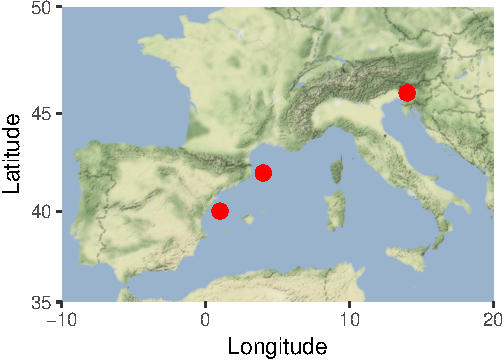
\includegraphics{proxymodelcomparison_files/figure-latex/map-1} \caption[Locations of 3 sample points]{Locations of 3 sample points.}\label{fig:map}
\end{marginfigure}

Create a matrix with the coordinates for the three locations of interest
in the west Mediterranean. We'll be focusing on large grid cell
averages, so the points do not have to be directly over land.

\begin{Shaded}
\begin{Highlighting}[]
\NormalTok{samp.pts <-}\StringTok{ }\KeywordTok{matrix}\NormalTok{(}\KeywordTok{c}\NormalTok{(}\DecValTok{1}\NormalTok{, }\DecValTok{40}\NormalTok{, }\DecValTok{4}\NormalTok{, }\DecValTok{42}\NormalTok{, }\DecValTok{14}\NormalTok{, }\DecValTok{46}\NormalTok{), }
                   \DataTypeTok{ncol =} \DecValTok{2}\NormalTok{, }\DataTypeTok{byrow =} \NormalTok{T)}
\end{Highlighting}
\end{Shaded}

\subsection{TraCE-21k}\label{trace-21k}

\begin{marginfigure}
\includegraphics{proxymodelcomparison_files/figure-latex/trace_map-1} \includegraphics{proxymodelcomparison_files/figure-latex/trace_map-2} \caption[TraCE21-k global precipitation and temperature]{TraCE21-k global precipitation and temperature}\label{fig:trace_map}
\end{marginfigure}

First, import data from the TraCE-21k paleoclimate simulation. Then
extract temperature and precipitation values at three locations in the
west Mediterranean. Use the \emph{brick} function from \textbf{raster}
to import decadal averages from the simulation. Put the coordinates for
the three locations in a matrix, and use that matrix to and
\textbf{raster's} \emph{extract} function to get the values from the
climate model brick. Convert the precipitation values to mm/year and
temperature values to degrees Celsius. Finally, name the columns for
each region appropriately.

Now pull all the TraCE data into one data frame, with one row per year,
and one column per variable/location combination. First \emph{rbind} the
two sets of TraCE data and \emph{transpose} the results, turning the 6
rows into 6 columns. Add a column for the Year (in ka BP), and use to
select only the entries earlier than 6,000 BP.

\begin{Shaded}
\begin{Highlighting}[]
\NormalTok{trace.dat <-}\StringTok{ }\KeywordTok{rbind}\NormalTok{(}
  \KeywordTok{brick}\NormalTok{(}\StringTok{'trace.01-36.22000BP.cam2.PRECT.22000BP_decavg_400BCE.nc'}\NormalTok{) %>%}
\StringTok{    }\NormalTok{raster::}\KeywordTok{extract}\NormalTok{(samp.pts) %>%}\StringTok{ }\CommentTok{# extract data at these coordinates}
\StringTok{    }\KeywordTok{multiply_by}\NormalTok{(}\FloatTok{3.154e+10}\NormalTok{), }\CommentTok{# convert to mm/year}
  \KeywordTok{brick}\NormalTok{(}\StringTok{'trace.01-36.22000BP.cam2.TREFHT.22000BP_decavg_400BCE.nc'}\NormalTok{) %>%}
\StringTok{    }\NormalTok{raster::}\KeywordTok{extract}\NormalTok{(samp.pts) %>%}\StringTok{ }
\StringTok{    }\KeywordTok{subtract}\NormalTok{(}\FloatTok{273.15}\NormalTok{)) %>%}\StringTok{ }\CommentTok{# convert from kelvin to C}
\StringTok{  }\NormalTok{t %>%}\StringTok{ }\CommentTok{# transpose}
\StringTok{  }\NormalTok{as.data.frame %>%}
\StringTok{  }\KeywordTok{set_colnames}\NormalTok{(}\KeywordTok{c}\NormalTok{(}\StringTok{'tmp,Southwest'}\NormalTok{, }\StringTok{'tmp,North Central'}\NormalTok{, }\StringTok{'tmp,Northeast'}\NormalTok{, }
                 \StringTok{'prc,Southwest'}\NormalTok{, }\StringTok{'prc,North Central'}\NormalTok{, }\StringTok{'prc,Northeast'}\NormalTok{)) %>%}
\StringTok{  }\KeywordTok{rownames_to_column}\NormalTok{(}\StringTok{'Year'}\NormalTok{) %>%}
\StringTok{  }\KeywordTok{mutate}\NormalTok{(}\DataTypeTok{Year =} \KeywordTok{as.numeric}\NormalTok{(}\KeywordTok{substring}\NormalTok{(Year, }\DecValTok{3}\NormalTok{))) %>%}
\StringTok{  }\KeywordTok{filter}\NormalTok{(Year >}\StringTok{ }\DecValTok{6}\NormalTok{) }\CommentTok{# get all the decades up to 6ka BP}
\end{Highlighting}
\end{Shaded}

\subsection{Trend Analysis}\label{trend-analysis}

Let's use the \textbf{EMD} package to calculate actual trend lines using
the empirical mode decomposition approach.

\begin{marginfigure}
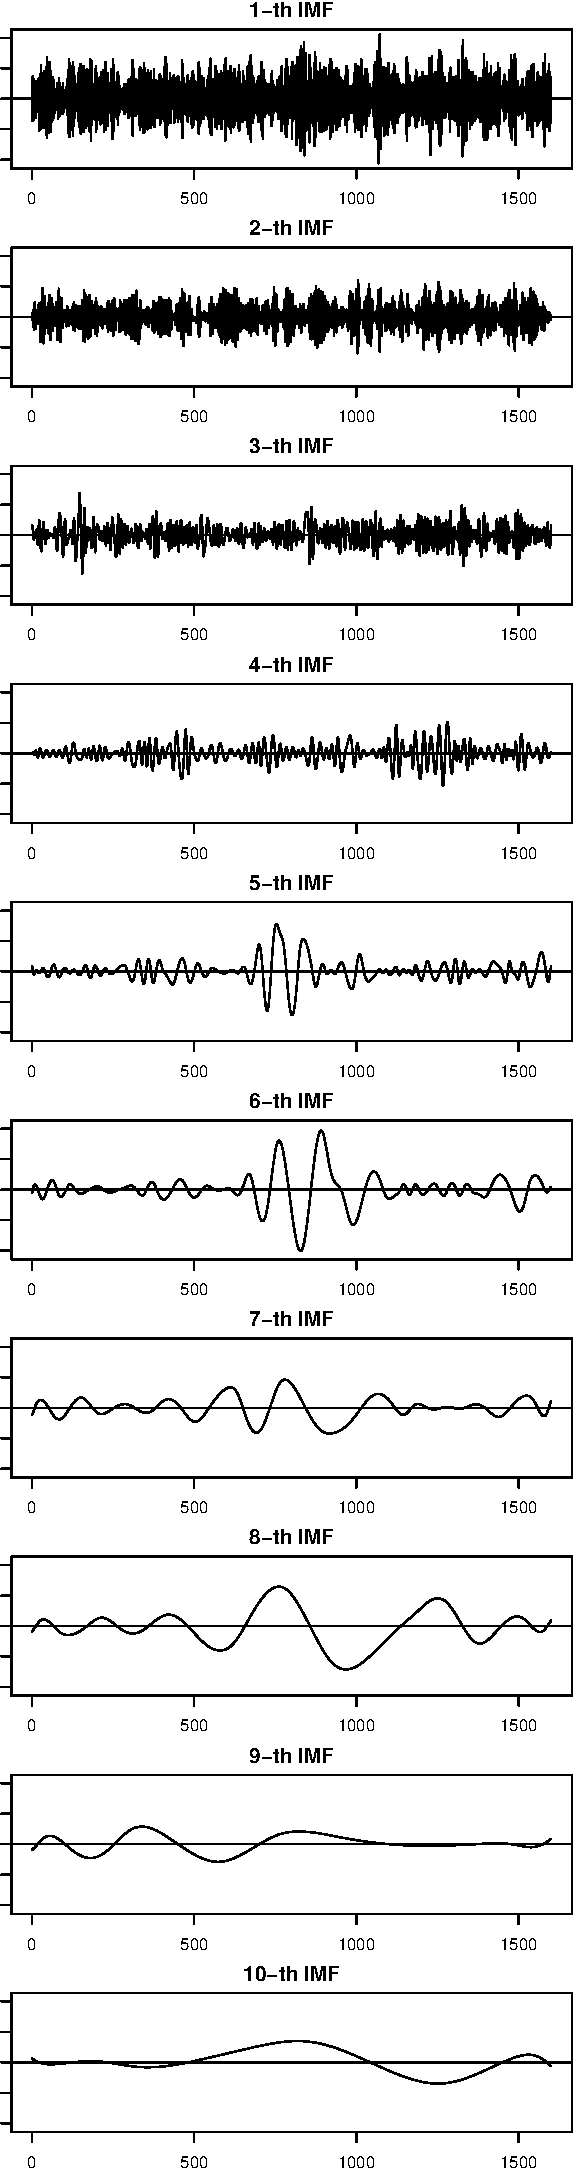
\includegraphics{proxymodelcomparison_files/figure-latex/unnamed-chunk-2-1} \caption[Empirical mode decomposition]{Empirical mode decomposition}\label{fig:unnamed-chunk-2}
\end{marginfigure}

Now organize the temperature and precipitation data to make plotting
easier using functions from \textbf{tidyr}.
\marginnote{Replace the variable names to make facet naming easier too.}

\begin{Shaded}
\begin{Highlighting}[]
\NormalTok{trace.plot <-}\StringTok{ }\NormalTok{trace.dat %>%}\StringTok{ }
\StringTok{  }\KeywordTok{gather}\NormalTok{(key, value, -}\StringTok{ }\NormalTok{Year) %>%}
\StringTok{  }\KeywordTok{separate}\NormalTok{(key, }\KeywordTok{c}\NormalTok{(}\StringTok{'Variable'}\NormalTok{, }\StringTok{'Region'}\NormalTok{), }\StringTok{','}\NormalTok{) %>%}
\StringTok{  }\KeywordTok{mutate}\NormalTok{(}\DataTypeTok{Variable =} \KeywordTok{ifelse}\NormalTok{(}
    \NormalTok{Variable ==}\StringTok{ 'tmp'}\NormalTok{, }\StringTok{'Temperature (°C)'}\NormalTok{, }\StringTok{'Precipitation (mm)'}\NormalTok{))}

\NormalTok{emd.res <-}\StringTok{ }\NormalTok{function(x) }\KeywordTok{emd}\NormalTok{(x)$residue}
\NormalTok{trace.emd <-}\StringTok{ }\NormalTok{trace.dat %>%}
\StringTok{  }\KeywordTok{mutate_at}\NormalTok{(}\KeywordTok{vars}\NormalTok{(-Year), emd.res) %>%}
\StringTok{  }\KeywordTok{gather}\NormalTok{(key, value, -}\StringTok{ }\NormalTok{Year) %>%}
\StringTok{  }\KeywordTok{separate}\NormalTok{(key, }\KeywordTok{c}\NormalTok{(}\StringTok{'Variable'}\NormalTok{, }\StringTok{'Region'}\NormalTok{), }\StringTok{','}\NormalTok{) %>%}
\StringTok{  }\KeywordTok{mutate}\NormalTok{(}\DataTypeTok{Variable =} \KeywordTok{ifelse}\NormalTok{(}
    \NormalTok{Variable ==}\StringTok{ 'tmp'}\NormalTok{, }\StringTok{'Temperature (°C)'}\NormalTok{, }\StringTok{'Precipitation (mm)'}\NormalTok{))}
\end{Highlighting}
\end{Shaded}

\subsection{Plotting}\label{plotting}

Plot everything with \textbf{ggplot2}.

\begin{marginfigure}
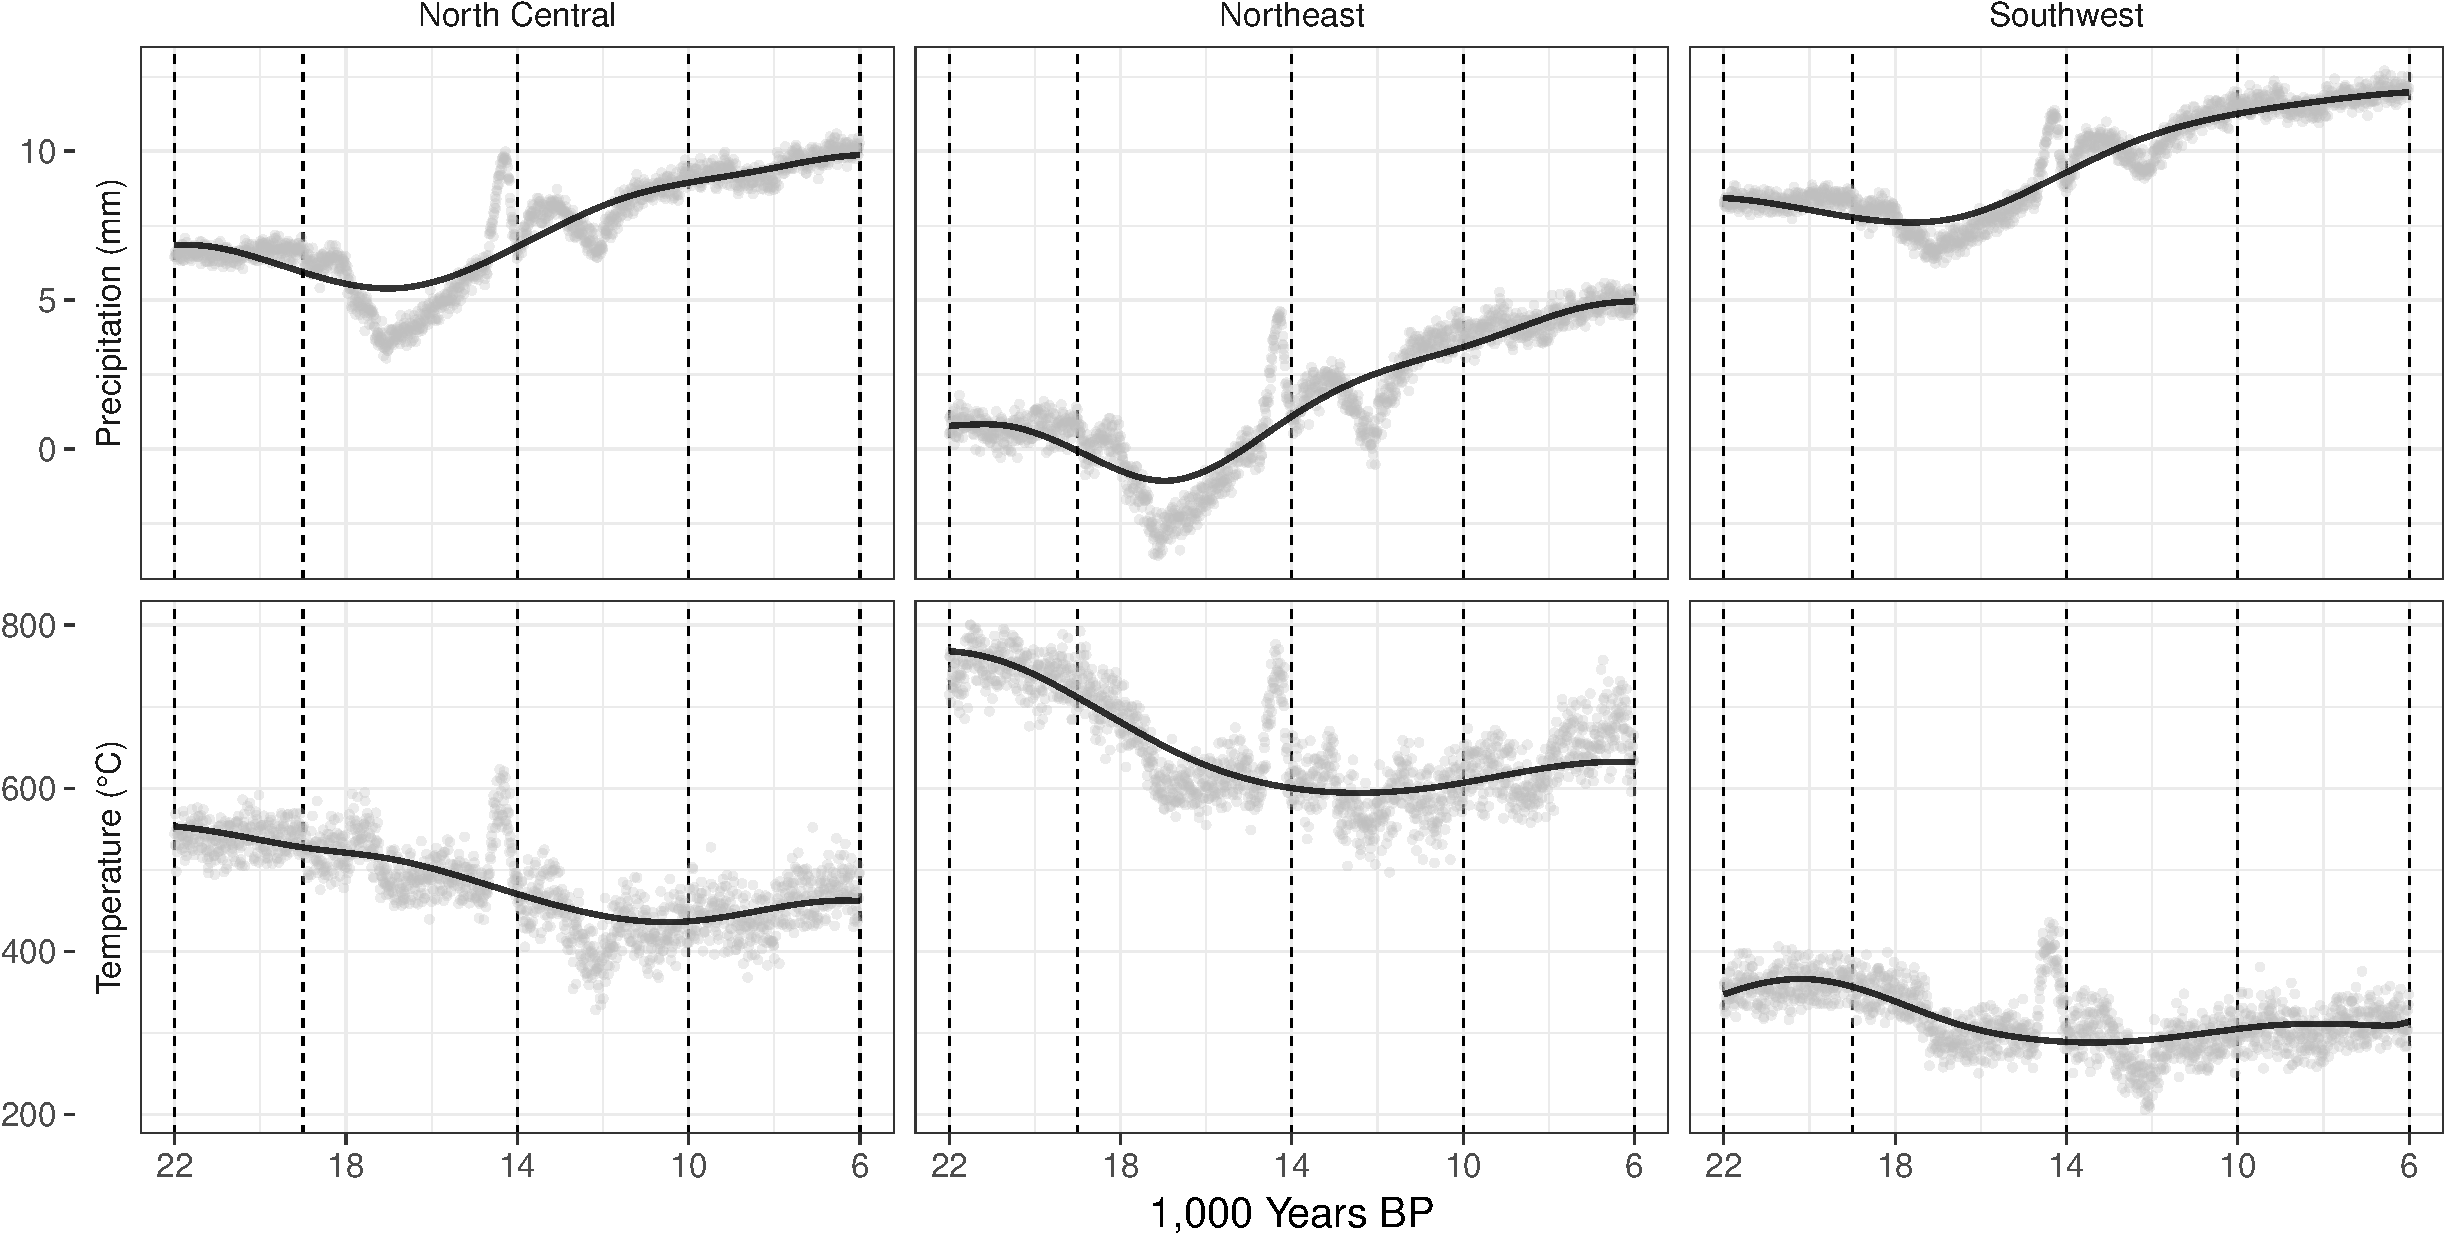
\includegraphics{proxymodelcomparison_files/figure-latex/bwplot-1} \caption[Black and white version]{Black and white version}\label{fig:bwplot}
\end{marginfigure}

\begin{Shaded}
\begin{Highlighting}[]
\KeywordTok{ggplot}\NormalTok{(}\DataTypeTok{data =} \NormalTok{trace.plot, }\KeywordTok{aes}\NormalTok{(}\DataTypeTok{x =} \NormalTok{Year, }\DataTypeTok{y =} \NormalTok{value)) +}
\StringTok{  }\KeywordTok{facet_grid}\NormalTok{(Variable ~}\StringTok{ }\NormalTok{Region, }\DataTypeTok{switch =} \StringTok{'y'}\NormalTok{, }\DataTypeTok{scale =} \StringTok{'free_y'}\NormalTok{) +}
\StringTok{  }\KeywordTok{geom_vline}\NormalTok{(}\DataTypeTok{xintercept =} \KeywordTok{c}\NormalTok{(}\DecValTok{22}\NormalTok{, }\DecValTok{19}\NormalTok{, }\DecValTok{14}\NormalTok{, }\DecValTok{10}\NormalTok{, }\DecValTok{6}\NormalTok{), }\DataTypeTok{lty =} \DecValTok{2}\NormalTok{) +}
\StringTok{  }\KeywordTok{geom_point}\NormalTok{(}\KeywordTok{aes}\NormalTok{(}\DataTypeTok{color =} \NormalTok{Variable), }\DataTypeTok{alpha =} \NormalTok{.}\DecValTok{3}\NormalTok{) +}
\StringTok{  }\KeywordTok{geom_line}\NormalTok{(}\DataTypeTok{data =} \NormalTok{trace.emd, }\DataTypeTok{size =} \FloatTok{1.2}\NormalTok{, }\DataTypeTok{color =} \StringTok{"black"}\NormalTok{, }\DataTypeTok{alpha =} \NormalTok{.}\DecValTok{8}\NormalTok{) +}
\StringTok{  }\KeywordTok{scale_x_reverse}\NormalTok{(}\DataTypeTok{breaks =} \KeywordTok{seq}\NormalTok{(}\DecValTok{6}\NormalTok{,}\DecValTok{22}\NormalTok{,}\DecValTok{4}\NormalTok{)) +}
\StringTok{  }\KeywordTok{labs}\NormalTok{(}\DataTypeTok{x =} \StringTok{'1,000 Years BP'}\NormalTok{, }\DataTypeTok{y =} \StringTok{''}\NormalTok{) +}
\StringTok{  }\KeywordTok{guides}\NormalTok{(}\DataTypeTok{color =} \StringTok{"none"}\NormalTok{) +}
\StringTok{  }\KeywordTok{theme_bw}\NormalTok{(}\DataTypeTok{base_size =} \DecValTok{20}\NormalTok{) +}
\StringTok{  }\KeywordTok{theme}\NormalTok{(}\DataTypeTok{strip.background  =} \KeywordTok{element_blank}\NormalTok{())}
\end{Highlighting}
\end{Shaded}

\begin{figure*}
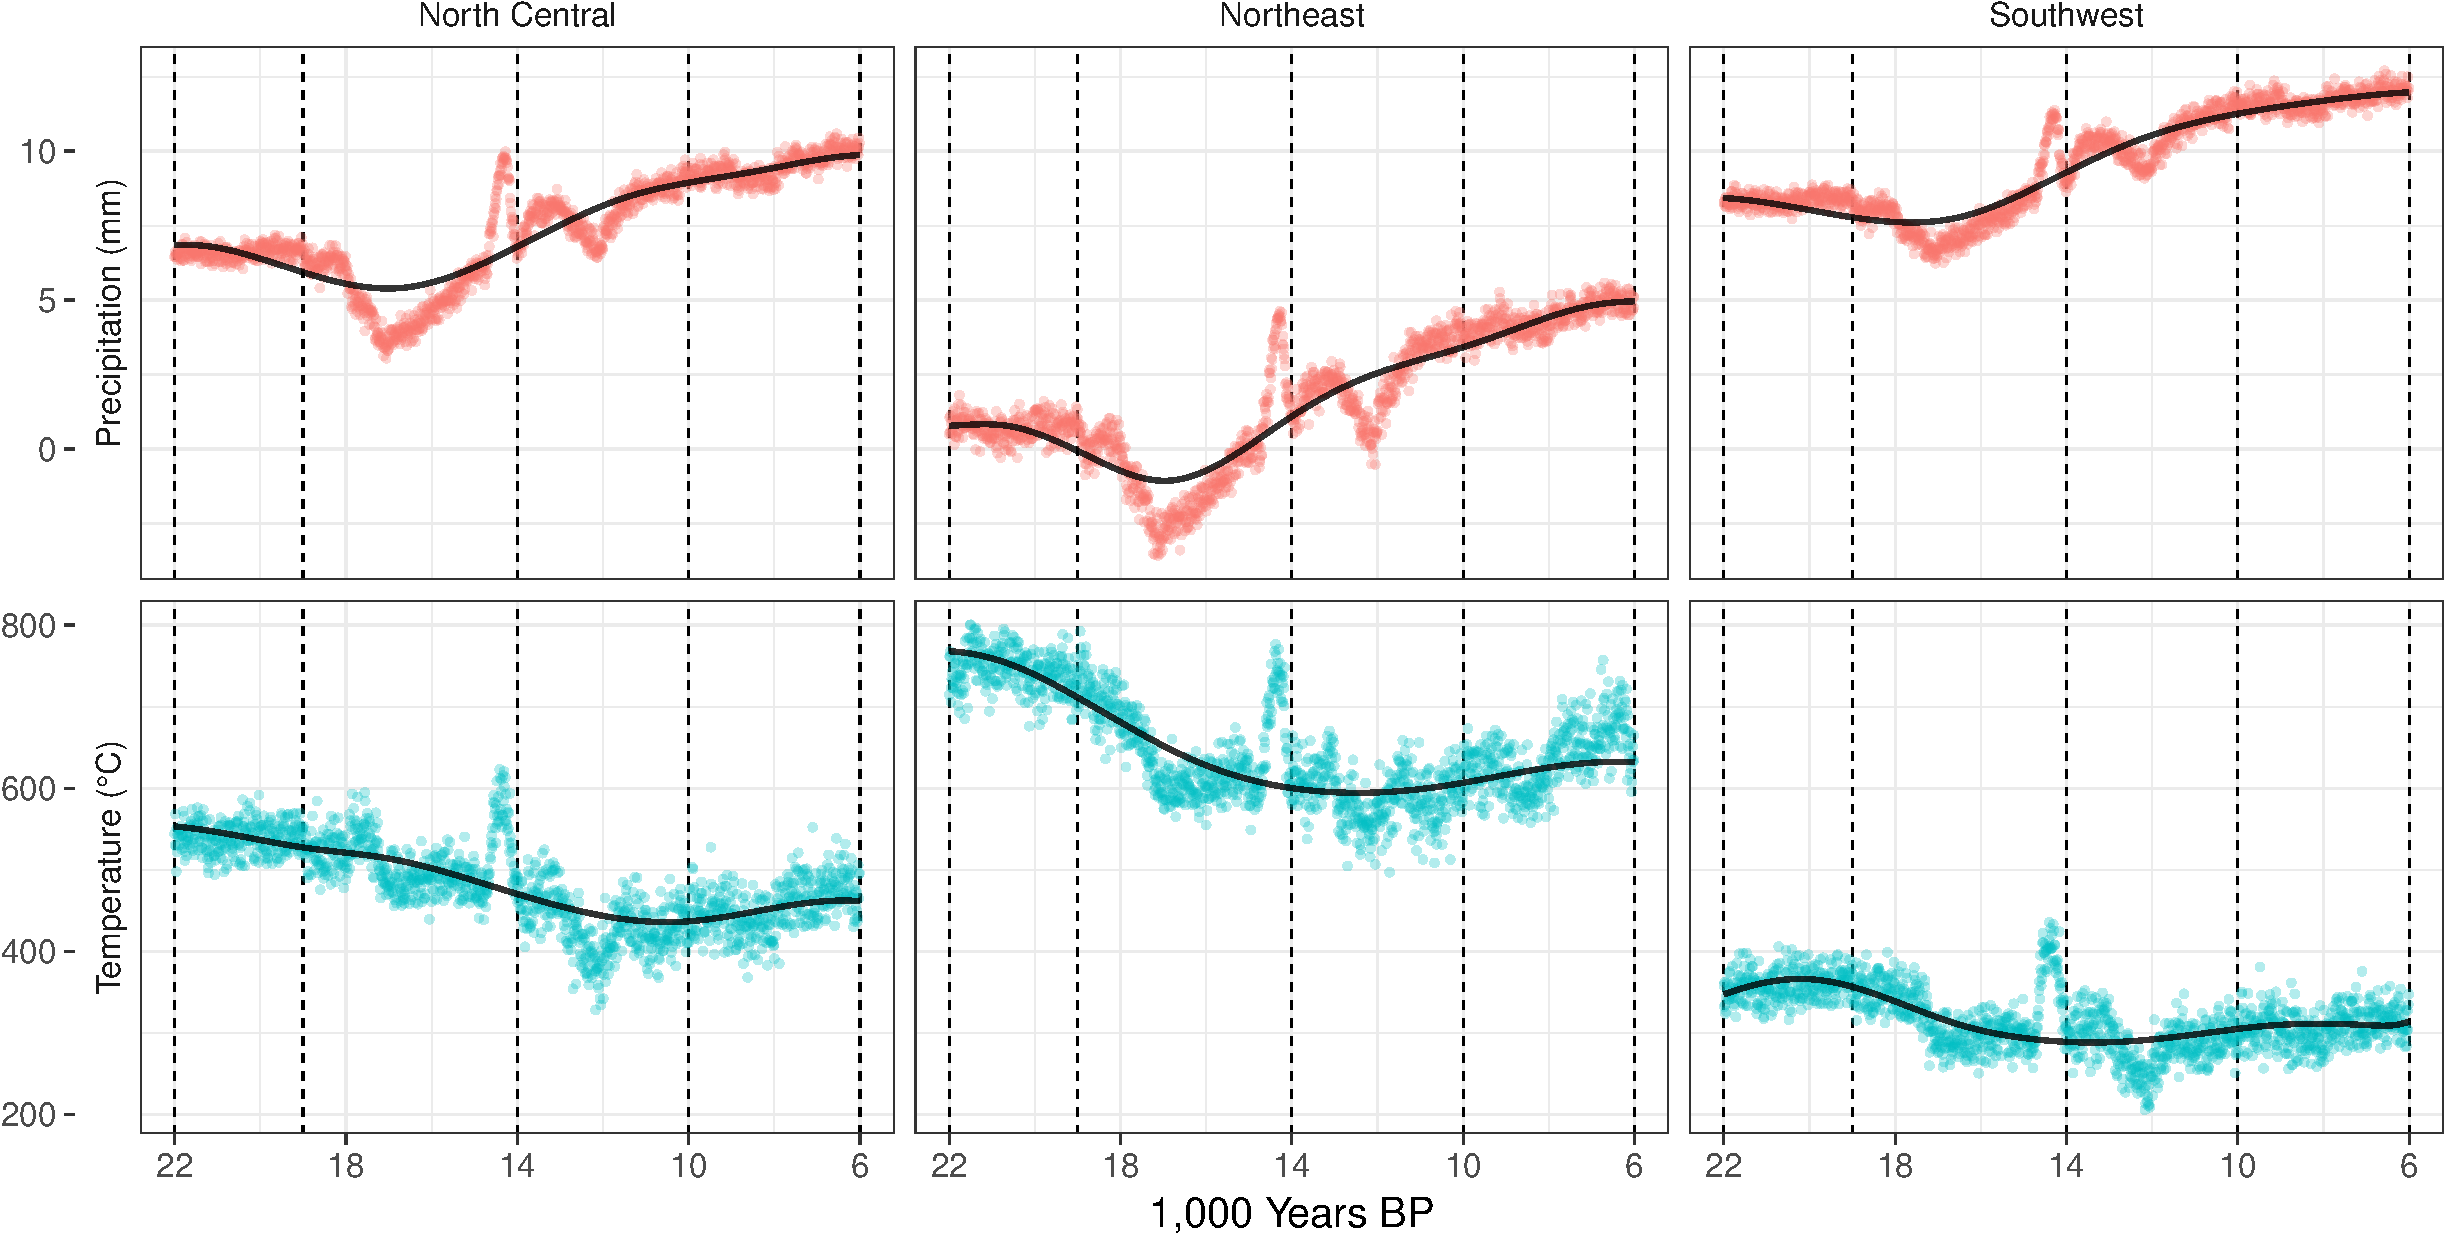
\includegraphics{proxymodelcomparison_files/figure-latex/mainplot-1} \end{figure*}

\subsection{Spatial patterns}\label{spatial-patterns}

Now let's import previously-downscaled ensemble equilibrium simulations
of the Last Glacial Maximum and Mid Holocene, to estimate how the
spatial patterns of climate variability have changed over time, and to
test for consistency with the transient TraCE simulation.

First import the downscaled data.

\begin{Shaded}
\begin{Highlighting}[]
\NormalTok{bbox <-}\StringTok{ }\KeywordTok{extent}\NormalTok{(}\KeywordTok{c}\NormalTok{(-}\DecValTok{10}\NormalTok{, }\DecValTok{20}\NormalTok{, }\DecValTok{35}\NormalTok{, }\DecValTok{47}\NormalTok{))}

\NormalTok{lgm.prc <-}\StringTok{ }\KeywordTok{brick}\NormalTok{(}\StringTok{'Downscaled/ensemble_prc_lgm.tif'}\NormalTok{) %>%}
\StringTok{  }\KeywordTok{crop}\NormalTok{(bbox)}
\NormalTok{mh.prc <-}\StringTok{ }\KeywordTok{brick}\NormalTok{(}\StringTok{'Downscaled/ensemble_prc_mh6k.tif'}\NormalTok{) %>%}
\StringTok{  }\KeywordTok{crop}\NormalTok{(bbox)}

\NormalTok{lgm.tmp <-}\StringTok{ }\KeywordTok{brick}\NormalTok{(}\StringTok{'Downscaled/ensemble_tmn_lgm.tif'}\NormalTok{) %>%}
\StringTok{  }\KeywordTok{crop}\NormalTok{(bbox) %>%}
\StringTok{  }\KeywordTok{add}\NormalTok{(}\KeywordTok{brick}\NormalTok{(}\StringTok{'Downscaled/ensemble_tmx_lgm.tif'}\NormalTok{) %>%}\StringTok{ }\KeywordTok{crop}\NormalTok{(bbox)) %>%}
\StringTok{  }\KeywordTok{divide_by}\NormalTok{(}\DecValTok{2}\NormalTok{)}
\NormalTok{mh.tmp <-}\StringTok{ }\KeywordTok{brick}\NormalTok{(}\StringTok{'Downscaled/ensemble_tmn_mh6k.tif'}\NormalTok{) %>%}
\StringTok{  }\KeywordTok{crop}\NormalTok{(bbox) %>%}
\StringTok{  }\KeywordTok{add}\NormalTok{(}\KeywordTok{brick}\NormalTok{(}\StringTok{'Downscaled/ensemble_tmx_mh6k.tif'}\NormalTok{) %>%}\StringTok{ }\KeywordTok{crop}\NormalTok{(bbox)) %>%}
\StringTok{  }\KeywordTok{divide_by}\NormalTok{(}\DecValTok{2}\NormalTok{)}
\end{Highlighting}
\end{Shaded}

Calculate changes in seasonal precipitation and temperature.

\begin{Shaded}
\begin{Highlighting}[]
\NormalTok{bySeason <-}\StringTok{ }\NormalTok{function(x, season, var)\{}
  \NormalTok{if(season ==}\StringTok{ 'djf'}\NormalTok{) \{ids <-}\StringTok{ }\KeywordTok{c}\NormalTok{(}\DecValTok{1}\NormalTok{,}\DecValTok{2}\NormalTok{,}\DecValTok{12}\NormalTok{)\}}
  \NormalTok{if(season ==}\StringTok{ 'jja'}\NormalTok{) \{ids <-}\StringTok{ }\KeywordTok{c}\NormalTok{(}\DecValTok{6}\NormalTok{,}\DecValTok{7}\NormalTok{,}\DecValTok{8}\NormalTok{)\}}
  
  \NormalTok{if(var ==}\StringTok{ 'tmp'}\NormalTok{) }\KeywordTok{return}\NormalTok{(}\KeywordTok{mean}\NormalTok{(x[[ids]]))}
  \NormalTok{if(var ==}\StringTok{ 'prc'}\NormalTok{) }\KeywordTok{return}\NormalTok{(}\KeywordTok{sum}\NormalTok{(x[[ids]]))}
\NormalTok{\}}

\NormalTok{prc.change.map <-}\StringTok{ }\KeywordTok{brick}\NormalTok{(}\KeywordTok{c}\NormalTok{(}
  \NormalTok{(}\KeywordTok{bySeason}\NormalTok{(mh.prc, }\StringTok{'djf'}\NormalTok{, }\StringTok{'prc'}\NormalTok{) -}\StringTok{ }\KeywordTok{bySeason}\NormalTok{(lgm.prc, }\StringTok{'djf'}\NormalTok{, }\StringTok{'prc'}\NormalTok{)) *}\StringTok{ }\DecValTok{100} \NormalTok{/}\StringTok{ }\KeywordTok{bySeason}\NormalTok{(lgm.prc, }\StringTok{'djf'}\NormalTok{, }\StringTok{'prc'}\NormalTok{),}
  \NormalTok{(}\KeywordTok{bySeason}\NormalTok{(mh.prc, }\StringTok{'jja'}\NormalTok{, }\StringTok{'prc'}\NormalTok{) -}\StringTok{ }\KeywordTok{bySeason}\NormalTok{(lgm.prc, }\StringTok{'jja'}\NormalTok{, }\StringTok{'prc'}\NormalTok{)) *}\StringTok{ }\DecValTok{100} \NormalTok{/}\StringTok{ }\KeywordTok{bySeason}\NormalTok{(lgm.prc, }\StringTok{'jja'}\NormalTok{, }\StringTok{'prc'}\NormalTok{)))}

\NormalTok{tmp.change.map <-}\StringTok{ }\KeywordTok{brick}\NormalTok{(}\KeywordTok{c}\NormalTok{(}
  \KeywordTok{bySeason}\NormalTok{(mh.tmp, }\StringTok{'djf'}\NormalTok{, }\StringTok{'tmp'}\NormalTok{) -}\StringTok{ }\KeywordTok{bySeason}\NormalTok{(lgm.tmp, }\StringTok{'djf'}\NormalTok{, }\StringTok{'tmp'}\NormalTok{),}
  \KeywordTok{bySeason}\NormalTok{(mh.tmp, }\StringTok{'jja'}\NormalTok{, }\StringTok{'tmp'}\NormalTok{) -}\StringTok{ }\KeywordTok{bySeason}\NormalTok{(lgm.tmp, }\StringTok{'jja'}\NormalTok{, }\StringTok{'tmp'}\NormalTok{)))}
\end{Highlighting}
\end{Shaded}

Plot the results

\begin{Shaded}
\begin{Highlighting}[]
\KeywordTok{levelplot}\NormalTok{(prc.change.map, }\DataTypeTok{margin =} \NormalTok{F, }\DataTypeTok{names.attr =} \KeywordTok{c}\NormalTok{(}\StringTok{'Winter'}\NormalTok{, }\StringTok{'Summer'}\NormalTok{),}
          \DataTypeTok{main =} \StringTok{'Precipitation Change (%)}\CharTok{\textbackslash{}n}\StringTok{ LGM to Mid Holocene'}\NormalTok{,}
          \DataTypeTok{par.settings =} \KeywordTok{PuOrTheme}\NormalTok{(), }
          \DataTypeTok{at =} \KeywordTok{seq}\NormalTok{(-}\DecValTok{100}\NormalTok{,}\DecValTok{100}\NormalTok{,}\DecValTok{10}\NormalTok{))}
\end{Highlighting}
\end{Shaded}

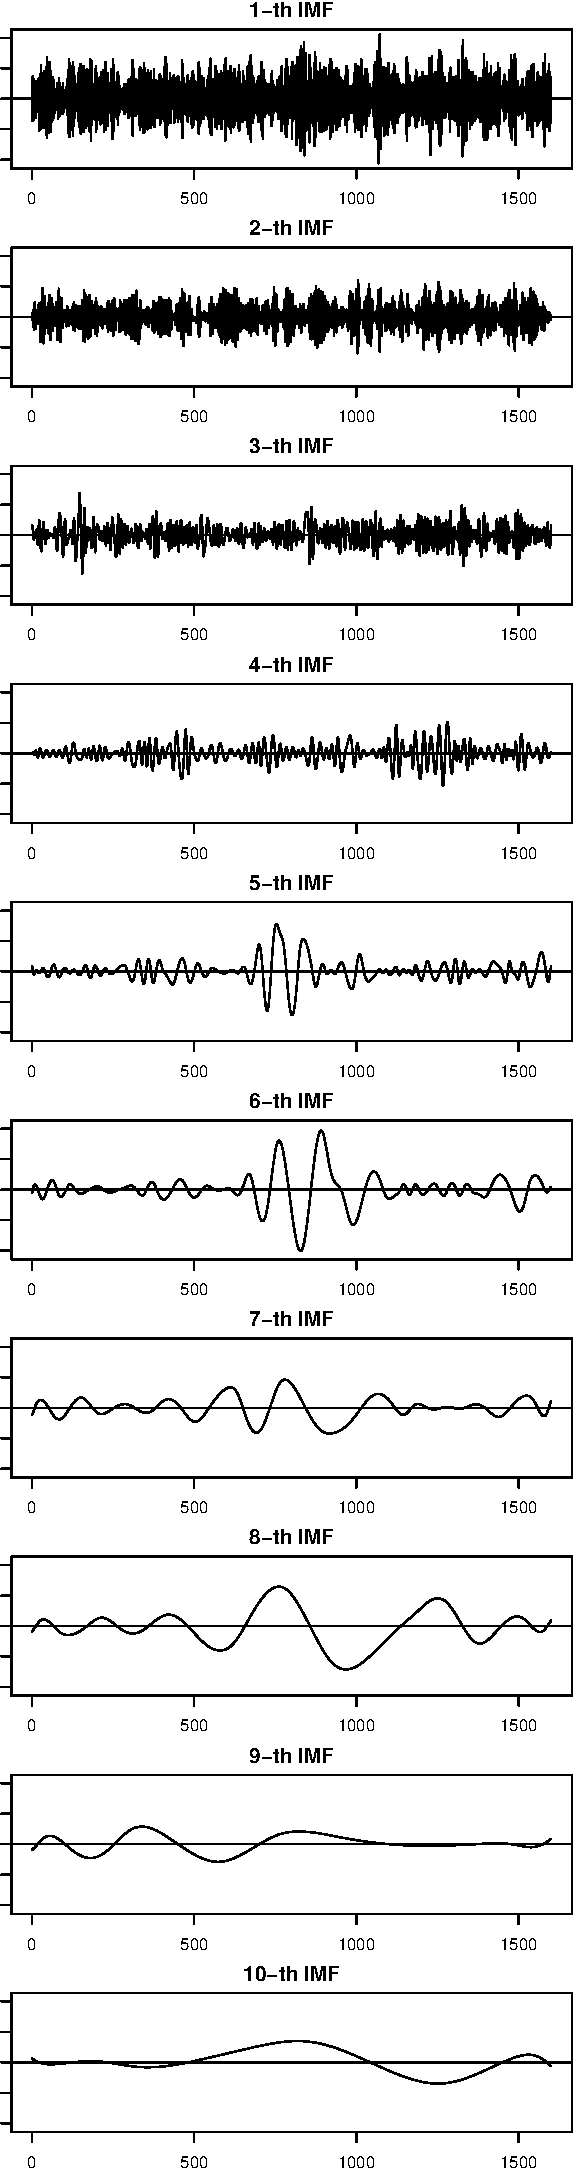
\includegraphics{proxymodelcomparison_files/figure-latex/unnamed-chunk-6-1}

\begin{Shaded}
\begin{Highlighting}[]
\KeywordTok{levelplot}\NormalTok{(tmp.change.map, }\DataTypeTok{margin =} \NormalTok{F, }\DataTypeTok{names.attr =} \KeywordTok{c}\NormalTok{(}\StringTok{'Winter'}\NormalTok{, }\StringTok{'Summer'}\NormalTok{), }
          \DataTypeTok{main =} \StringTok{'Temperature Change}\CharTok{\textbackslash{}n}\StringTok{ LGM to Mid Holocene'}\NormalTok{,}
          \DataTypeTok{par.settings =} \KeywordTok{BuRdTheme}\NormalTok{(),}
          \DataTypeTok{at =} \KeywordTok{seq}\NormalTok{(-}\DecValTok{20}\NormalTok{,}\DecValTok{20}\NormalTok{,}\DecValTok{2}\NormalTok{))}
\end{Highlighting}
\end{Shaded}

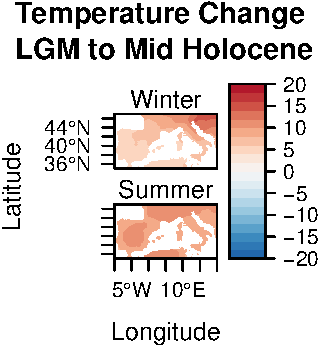
\includegraphics{proxymodelcomparison_files/figure-latex/unnamed-chunk-6-2}

Now we can calculate changes in seasonality. For temperature, this is
just the standard deviation of all 12 monthly averages. For
precipitation, we will use the coefficient of variation.

\begin{Shaded}
\begin{Highlighting}[]
\NormalTok{tmp.seasonality <-}\StringTok{ }\KeywordTok{calc}\NormalTok{(mh.tmp, sd) -}\StringTok{ }\KeywordTok{calc}\NormalTok{(lgm.tmp, sd)}
\NormalTok{prc.seasonality <-}\StringTok{ }\KeywordTok{cv}\NormalTok{(mh.prc) -}\StringTok{ }\KeywordTok{cv}\NormalTok{(lgm.prc)}
\end{Highlighting}
\end{Shaded}

Plot the results.

\begin{Shaded}
\begin{Highlighting}[]
\KeywordTok{levelplot}\NormalTok{(tmp.seasonality, }\DataTypeTok{margin =} \NormalTok{F, }
          \DataTypeTok{main =} \StringTok{'Change in temperature seasonality (SD)}\CharTok{\textbackslash{}n}\StringTok{ LGM to Mid Holocene'}\NormalTok{, }
          \DataTypeTok{par.settings =} \KeywordTok{BuRdTheme}\NormalTok{(), }
          \DataTypeTok{at =} \KeywordTok{seq}\NormalTok{(-}\DecValTok{4}\NormalTok{, }\DecValTok{4}\NormalTok{, .}\DecValTok{4}\NormalTok{))}
\end{Highlighting}
\end{Shaded}

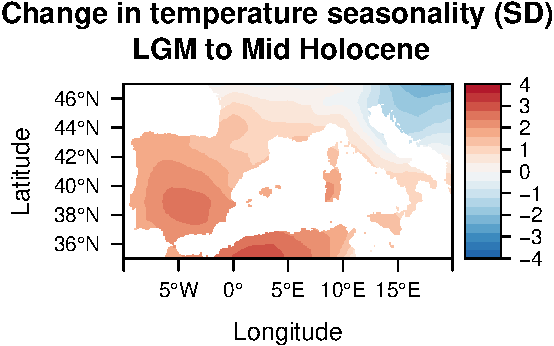
\includegraphics{proxymodelcomparison_files/figure-latex/unnamed-chunk-8-1}

\begin{Shaded}
\begin{Highlighting}[]
\KeywordTok{levelplot}\NormalTok{(prc.seasonality, }\DataTypeTok{margin =} \NormalTok{F, }
          \DataTypeTok{main =} \StringTok{'Change in precipitation seasonality (CV)}\CharTok{\textbackslash{}n}\StringTok{ LGM to Mid Holocene'}\NormalTok{, }
          \DataTypeTok{par.settings =} \KeywordTok{BuRdTheme}\NormalTok{(), }
          \DataTypeTok{at =} \KeywordTok{seq}\NormalTok{(-}\DecValTok{50}\NormalTok{, }\DecValTok{50}\NormalTok{, }\DecValTok{5}\NormalTok{))}
\end{Highlighting}
\end{Shaded}

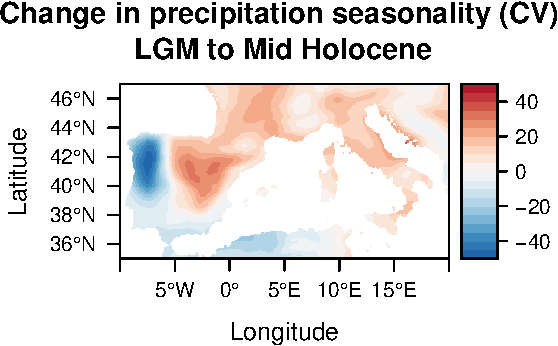
\includegraphics{proxymodelcomparison_files/figure-latex/unnamed-chunk-8-2}

What about changes in spatial hetergeneity?

\begin{Shaded}
\begin{Highlighting}[]
\NormalTok{wts <-}\StringTok{ }\KeywordTok{matrix}\NormalTok{(}\KeywordTok{c}\NormalTok{(}\DecValTok{0}\NormalTok{,}\DecValTok{0}\NormalTok{,}\DecValTok{1}\NormalTok{,}\DecValTok{0}\NormalTok{,}\DecValTok{0}\NormalTok{,}\DecValTok{0}\NormalTok{,}\DecValTok{1}\NormalTok{,}\DecValTok{1}\NormalTok{,}\DecValTok{1}\NormalTok{,}\DecValTok{0}\NormalTok{,}\DecValTok{1}\NormalTok{,}\DecValTok{1}\NormalTok{,}\DecValTok{1}\NormalTok{,}\DecValTok{1}\NormalTok{,}\DecValTok{1}\NormalTok{,}\DecValTok{0}\NormalTok{,}\DecValTok{1}\NormalTok{,}\DecValTok{1}\NormalTok{,}\DecValTok{1}\NormalTok{,}\DecValTok{0}\NormalTok{,}\DecValTok{0}\NormalTok{,}\DecValTok{0}\NormalTok{,}\DecValTok{1}\NormalTok{,}\DecValTok{0}\NormalTok{,}\DecValTok{0}\NormalTok{), }\DataTypeTok{nrow =} \DecValTok{5}\NormalTok{)}

\NormalTok{tmp.hetero <-}\StringTok{ }\KeywordTok{brick}\NormalTok{(}\KeywordTok{c}\NormalTok{(}
  \KeywordTok{bySeason}\NormalTok{(mh.tmp, }\StringTok{'djf'}\NormalTok{, }\StringTok{'tmp'}\NormalTok{) %>%}
\StringTok{    }\KeywordTok{focal}\NormalTok{(}\DataTypeTok{w =} \NormalTok{wts, sd, }\DataTypeTok{na.rm =} \NormalTok{T) %>%}
\StringTok{    }\KeywordTok{subtract}\NormalTok{(}
      \KeywordTok{bySeason}\NormalTok{(lgm.tmp, }\StringTok{'djf'}\NormalTok{, }\StringTok{'tmp'}\NormalTok{) %>%}\StringTok{ }
\StringTok{        }\KeywordTok{focal}\NormalTok{(}\DataTypeTok{w =} \NormalTok{wts, sd, }\DataTypeTok{na.rm =} \NormalTok{T)),}
  \KeywordTok{bySeason}\NormalTok{(mh.tmp, }\StringTok{'jja'}\NormalTok{, }\StringTok{'tmp'}\NormalTok{) %>%}
\StringTok{    }\KeywordTok{focal}\NormalTok{(}\DataTypeTok{w =} \NormalTok{wts, sd, }\DataTypeTok{na.rm =} \NormalTok{T) %>%}
\StringTok{    }\KeywordTok{subtract}\NormalTok{(}
      \KeywordTok{bySeason}\NormalTok{(lgm.tmp, }\StringTok{'jja'}\NormalTok{, }\StringTok{'tmp'}\NormalTok{) %>%}\StringTok{ }
\StringTok{        }\KeywordTok{focal}\NormalTok{(}\DataTypeTok{w =} \NormalTok{wts, sd, }\DataTypeTok{na.rm =} \NormalTok{T)))) %>%}
\StringTok{  }\KeywordTok{mask}\NormalTok{(mh.tmp[[}\DecValTok{1}\NormalTok{]]) }\CommentTok{# clip buffer added by window}
  
\KeywordTok{levelplot}\NormalTok{(tmp.hetero, }\DataTypeTok{margin =} \NormalTok{F, }\DataTypeTok{names.attr =} \KeywordTok{c}\NormalTok{(}\StringTok{'Winter'}\NormalTok{, }\StringTok{'Summer'}\NormalTok{), }
          \DataTypeTok{main =} \StringTok{'Temperature heterogeneity (SD in 25km radius) change}\CharTok{\textbackslash{}n}\StringTok{ LGM to Mid Holocene'}\NormalTok{,}
          \DataTypeTok{par.settings =} \KeywordTok{BuRdTheme}\NormalTok{(), }\DataTypeTok{at =} \KeywordTok{seq}\NormalTok{(-}\DecValTok{10}\NormalTok{, }\DecValTok{10}\NormalTok{, }\DecValTok{1}\NormalTok{))}
\end{Highlighting}
\end{Shaded}

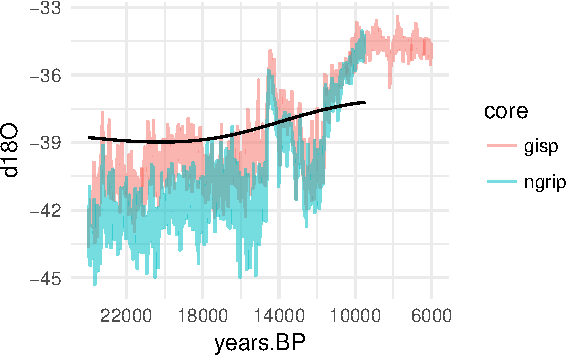
\includegraphics{proxymodelcomparison_files/figure-latex/unnamed-chunk-9-1}
Same for precipitaiton.

\begin{Shaded}
\begin{Highlighting}[]
\NormalTok{prc.hetero <-}\StringTok{ }\KeywordTok{brick}\NormalTok{(}\KeywordTok{c}\NormalTok{(}
  \KeywordTok{bySeason}\NormalTok{(mh.prc, }\StringTok{'djf'}\NormalTok{, }\StringTok{'prc'}\NormalTok{) %>%}
\StringTok{    }\KeywordTok{focal}\NormalTok{(}\DataTypeTok{w =} \NormalTok{wts, sd, }\DataTypeTok{na.rm =} \NormalTok{T) %>%}
\StringTok{    }\KeywordTok{subtract}\NormalTok{(}
      \KeywordTok{bySeason}\NormalTok{(lgm.prc, }\StringTok{'djf'}\NormalTok{, }\StringTok{'prc'}\NormalTok{) %>%}\StringTok{ }
\StringTok{        }\KeywordTok{focal}\NormalTok{(}\DataTypeTok{w =} \NormalTok{wts, sd, }\DataTypeTok{na.rm =} \NormalTok{T)),}
  \KeywordTok{bySeason}\NormalTok{(mh.prc, }\StringTok{'jja'}\NormalTok{, }\StringTok{'prc'}\NormalTok{) %>%}
\StringTok{    }\KeywordTok{focal}\NormalTok{(}\DataTypeTok{w =} \NormalTok{wts, sd, }\DataTypeTok{na.rm =} \NormalTok{T) %>%}
\StringTok{    }\KeywordTok{subtract}\NormalTok{(}
      \KeywordTok{bySeason}\NormalTok{(lgm.prc, }\StringTok{'jja'}\NormalTok{, }\StringTok{'prc'}\NormalTok{) %>%}\StringTok{ }
\StringTok{        }\KeywordTok{focal}\NormalTok{(}\DataTypeTok{w =} \NormalTok{wts, sd, }\DataTypeTok{na.rm =} \NormalTok{T)))) %>%}
\StringTok{  }\KeywordTok{mask}\NormalTok{(mh.prc[[}\DecValTok{1}\NormalTok{]]) }\CommentTok{# clip buffer added by window}
  
  
\KeywordTok{levelplot}\NormalTok{(prc.hetero, }\DataTypeTok{margin =} \NormalTok{F, }\DataTypeTok{names.attr =} \KeywordTok{c}\NormalTok{(}\StringTok{'Winter'}\NormalTok{, }\StringTok{'Summer'}\NormalTok{), }
          \DataTypeTok{main =} \StringTok{'Precipitation heterogeneity (SD in 25km radius) change}\CharTok{\textbackslash{}n}\StringTok{ LGM to Mid Holocene'}\NormalTok{,}
          \DataTypeTok{par.settings =} \KeywordTok{BuRdTheme}\NormalTok{(), }\DataTypeTok{at =} \KeywordTok{seq}\NormalTok{(-}\DecValTok{500}\NormalTok{, }\DecValTok{500}\NormalTok{, }\DecValTok{50}\NormalTok{))}
\end{Highlighting}
\end{Shaded}

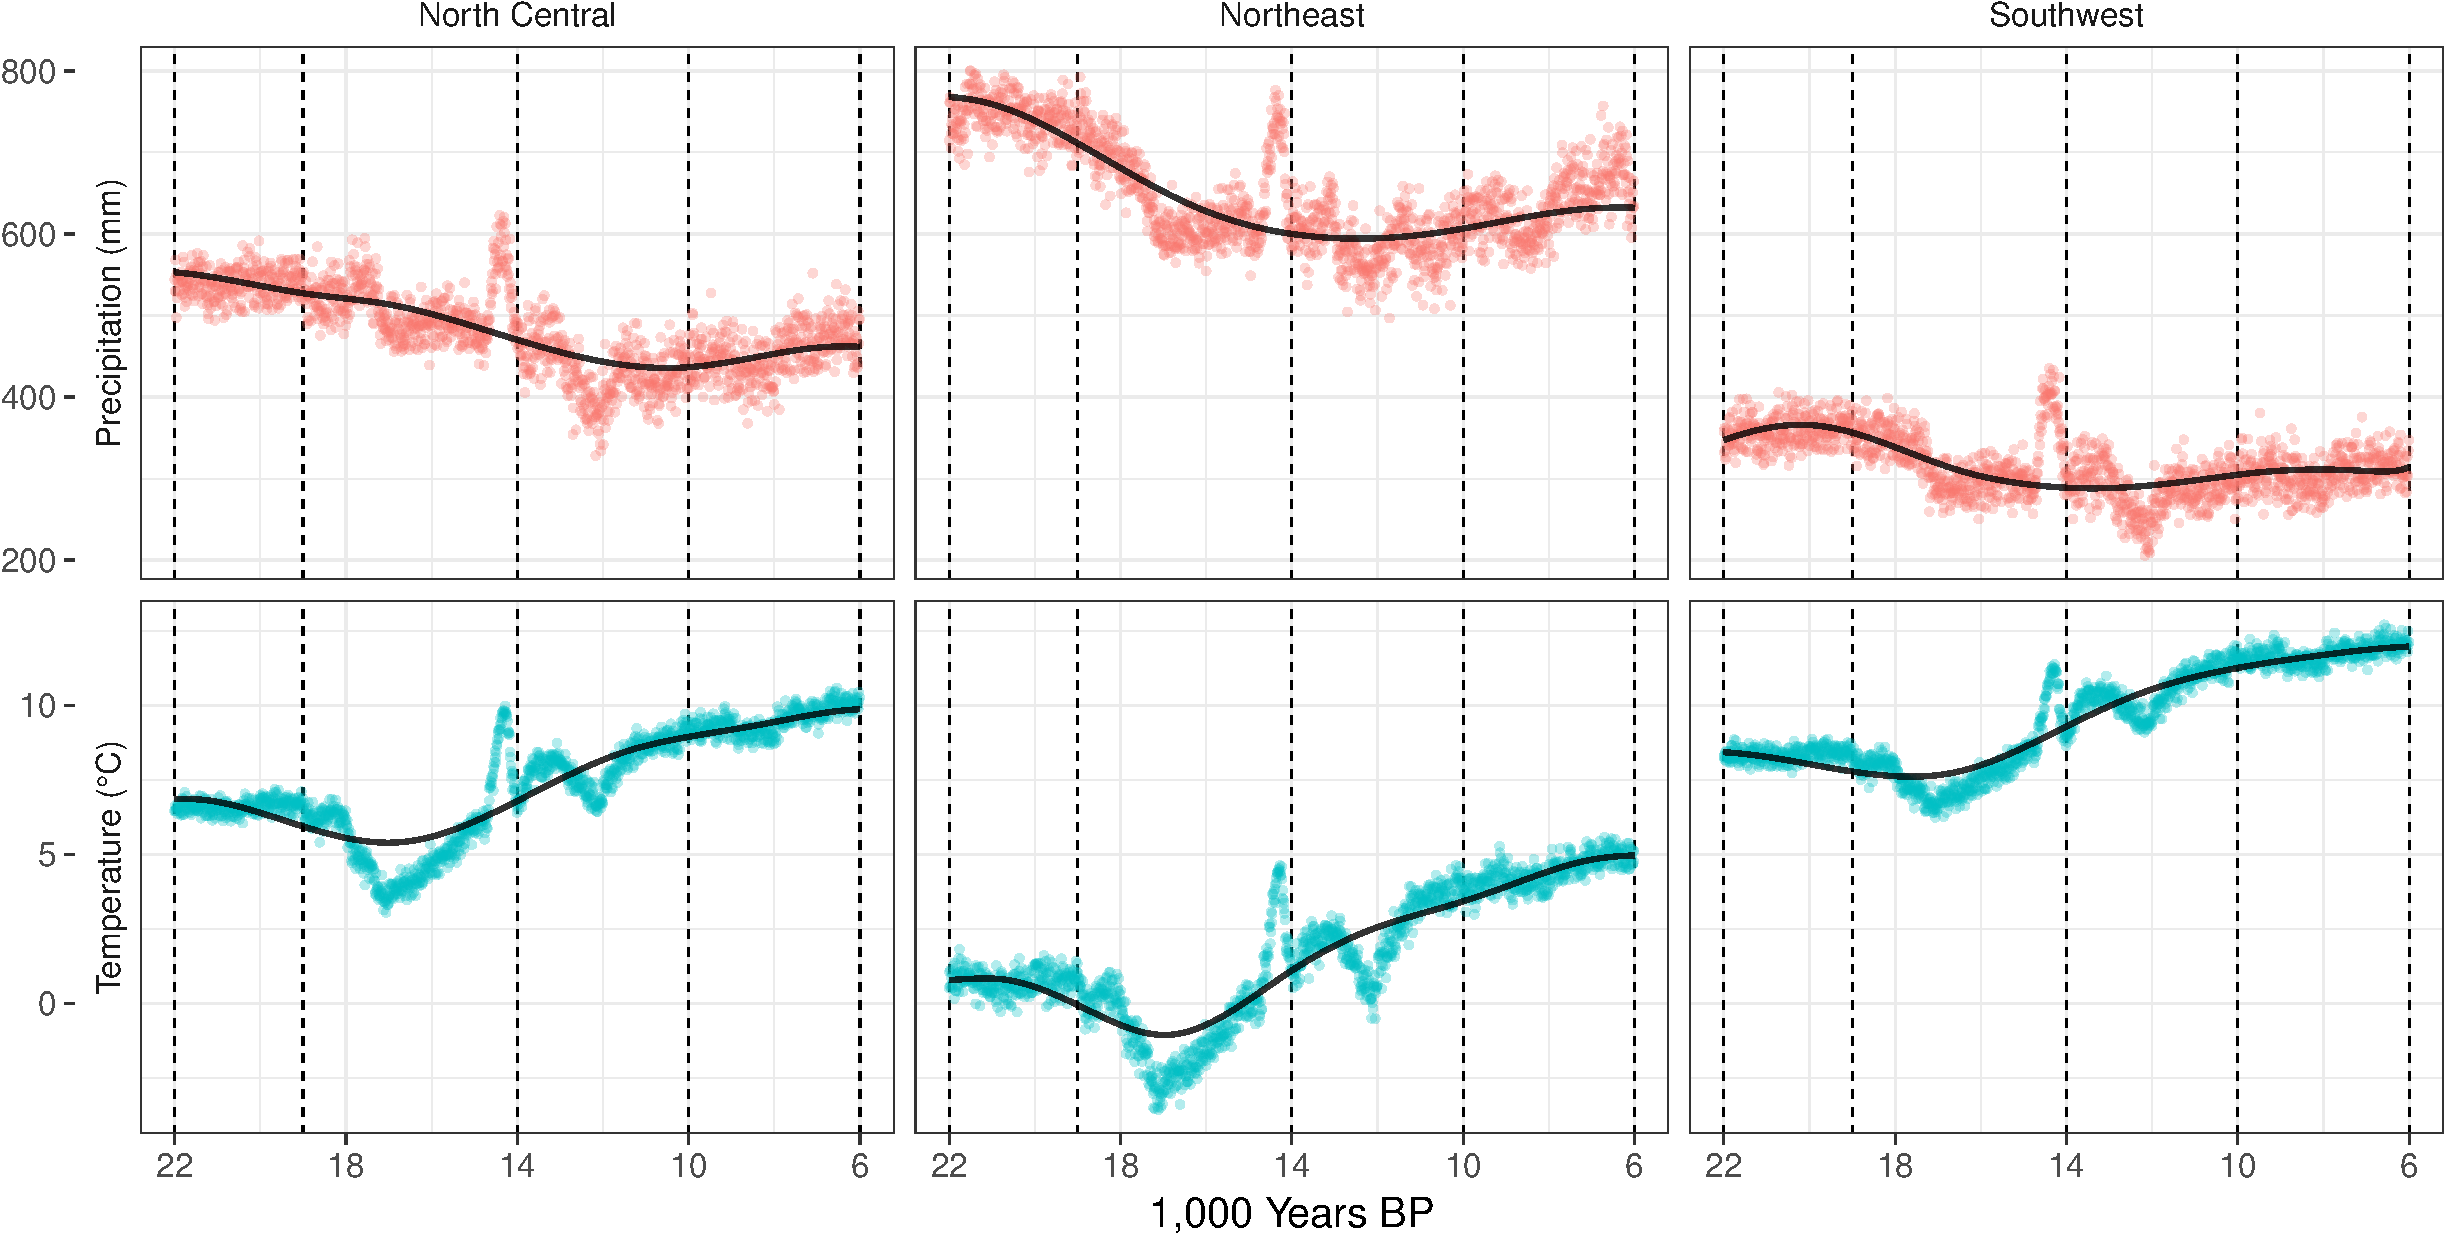
\includegraphics{proxymodelcomparison_files/figure-latex/unnamed-chunk-10-1}

\marginnote{Compare these with raw gcm outputs to check the added value of SDM}

\section{Proxy records}\label{proxy-records}

Get ice core data.

\begin{Shaded}
\begin{Highlighting}[]
\NormalTok{core.dat <-}\StringTok{ }\KeywordTok{read_csv}\NormalTok{(}\StringTok{'icecores_newdates.csv'}\NormalTok{) %>%}
\StringTok{  }\KeywordTok{transmute}\NormalTok{(years.BP, }\DataTypeTok{ngrip =}  \NormalTok{d18O.NGRIP2.ppt, }\DataTypeTok{gisp =} \NormalTok{d18O.GISP2.ppt) %>%}
\StringTok{  }\KeywordTok{filter}\NormalTok{(years.BP <}\StringTok{ }\DecValTok{24000} \NormalTok{&}\StringTok{ }\NormalTok{years.BP >=}\DecValTok{6000}\NormalTok{)}
\end{Highlighting}
\end{Shaded}

\begin{verbatim}
## Warning: Missing column names filled in:
## 'X1' [1]
\end{verbatim}

Plot it

\begin{Shaded}
\begin{Highlighting}[]
\NormalTok{core.plot <-}\StringTok{ }\KeywordTok{gather}\NormalTok{(core.dat, }\StringTok{'core'}\NormalTok{, }\StringTok{'d18O'}\NormalTok{, }\DecValTok{2}\NormalTok{:}\DecValTok{3}\NormalTok{)}

\KeywordTok{ggplot}\NormalTok{(core.plot, }\KeywordTok{aes}\NormalTok{(}\DataTypeTok{x =} \NormalTok{years.BP, }\DataTypeTok{y =} \NormalTok{d18O, }\DataTypeTok{color =} \NormalTok{core)) +}
\StringTok{  }\KeywordTok{geom_line}\NormalTok{(}\DataTypeTok{alpha =} \NormalTok{.}\DecValTok{54}\NormalTok{) +}
\StringTok{  }\KeywordTok{geom_smooth}\NormalTok{() +}
\StringTok{  }\KeywordTok{scale_x_reverse}\NormalTok{(}\DataTypeTok{breaks =} \KeywordTok{seq}\NormalTok{(}\DecValTok{6000}\NormalTok{,}\DecValTok{22000}\NormalTok{,}\DecValTok{4000}\NormalTok{)) +}
\StringTok{  }\KeywordTok{theme_minimal}\NormalTok{()}
\end{Highlighting}
\end{Shaded}

\begin{verbatim}
## `geom_smooth()` using method = 'gam'
\end{verbatim}

\begin{verbatim}
## Warning: Removed 367 rows containing non-finite
## values (stat_smooth).
\end{verbatim}

\begin{verbatim}
## Warning: Removed 348 rows containing missing
## values (geom_path).
\end{verbatim}

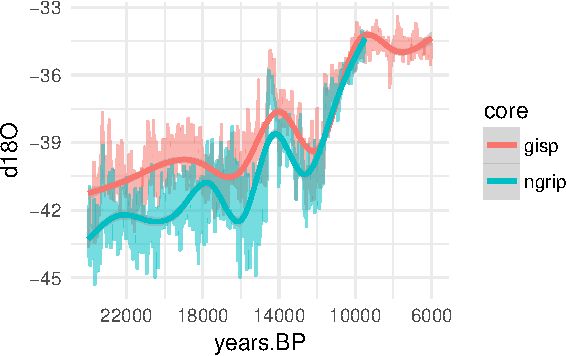
\includegraphics{proxymodelcomparison_files/figure-latex/unnamed-chunk-12-1}

\subsection{Detrending}\label{detrending}

\begin{Shaded}
\begin{Highlighting}[]
\NormalTok{cores <-}\StringTok{ }\NormalTok{core.dat %>%}\StringTok{ }\NormalTok{na.omit}
\NormalTok{core.emd.plot <-}\StringTok{ }\KeywordTok{emd}\NormalTok{(cores$gisp, cores$years.BP)$residue %>%}\StringTok{ }
\StringTok{  }\KeywordTok{data_frame}\NormalTok{(}\DataTypeTok{d18O =} \NormalTok{., }\DataTypeTok{years.BP =} \NormalTok{cores$years.BP)}
\end{Highlighting}
\end{Shaded}

\begin{Shaded}
\begin{Highlighting}[]
\KeywordTok{ggplot}\NormalTok{(core.plot, }\KeywordTok{aes}\NormalTok{(}\DataTypeTok{x =} \NormalTok{years.BP, }\DataTypeTok{y =} \NormalTok{d18O)) +}
\StringTok{  }\KeywordTok{geom_line}\NormalTok{(}\KeywordTok{aes}\NormalTok{(}\DataTypeTok{color =} \NormalTok{core), }\DataTypeTok{alpha =} \NormalTok{.}\DecValTok{54}\NormalTok{) +}
\StringTok{  }\KeywordTok{geom_line}\NormalTok{(}\DataTypeTok{data =} \NormalTok{core.emd.plot) +}
\StringTok{  }\KeywordTok{scale_x_reverse}\NormalTok{(}\DataTypeTok{breaks =} \KeywordTok{seq}\NormalTok{(}\DecValTok{6000}\NormalTok{,}\DecValTok{22000}\NormalTok{,}\DecValTok{4000}\NormalTok{)) +}
\StringTok{  }\KeywordTok{theme_minimal}\NormalTok{()}
\end{Highlighting}
\end{Shaded}

\begin{verbatim}
## Warning: Removed 348 rows containing missing
## values (geom_path).
\end{verbatim}

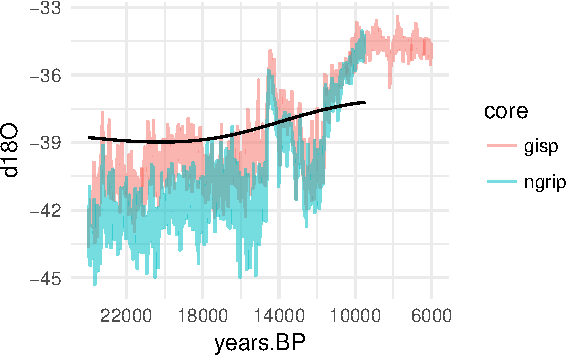
\includegraphics{proxymodelcomparison_files/figure-latex/unnamed-chunk-14-1}



\end{document}
